
\section{Linzalar beradigan tasvirlar}

\begin{enumerate}
\item Rasmda linza, buyum, linzaning bosh optik o‘qi va fokuslari tasvirlangan. Shu vaziyatdagi buyumning tasviri qanday bo‘ladi?

\begin{tikzpicture}[>=latex]
    \draw (-4,0) -- (4,0); \draw[thick, <->] (0,-2) -- (0,2);
    \foreach \x/\l in {-3/2F, -1.5/F, 1.5/F, 3/2F} {\draw (\x,0.1) -- (\x,-0.1) node[below] {\l};}
    \draw[ultra thick, ->] (-0.7,0) node[below] {A} -- (-0.7,1.2) node[above] {B};
\end{tikzpicture}

\begin{enumerate}[label=\Alph*)]
\item haqiqiy, kichiklashgan va teskari.
\item haqiqiy, kattalashgan va to‘g‘ri.
\item mavhum, kichiklashgan va teskari.
\item mavhum, kattalashgan va to‘g‘ri.
\end{enumerate}

\item Buyum qavariq linza va uning fokusi orasida joylashgan bo‘lsa, uning tasviri qanday va qayerda bo‘ladi?

\begin{enumerate}[label=\Alph*)]
\item bunday joylashishda tasvir hosil bo‘lmaydi.
\item haqiqiy, teskari, kichiklashgan, linzaning buyum yo‘q tomonida.
\item mavhum, teskari, kattalashgan, linzaning buyum yo‘q tomonida.
\item mavhum, to‘g‘ri, kattalashgan, linzaning buyum joylashgan tomonida.
\end{enumerate}

\item Yig‘uvchi linza yordamida mavhum tasvir hosil qilish uchun buyum \dots joylashgan bo‘lishi kerak. Nuqtalar o‘rniga to‘g‘risini tanlab qo‘ying.

\begin{enumerate}[label=\Alph*)]
\item linza fokusida.
\item linza va fokus orasida.
\item linza va ikkilangan fokus orasida.
\item ikkilangan fokusdan keyin.
\end{enumerate}

\item Buyum yig‘uvchi linzadan qanday masofada joylashgan bo‘lsa, mavhum, to‘g‘ri bo‘ladi?

\begin{enumerate}[label=\Alph*)]
\item $d<F$
\item $d>F$
\item $d>2F$
\item $d=2F$
\end{enumerate}

\item Quyidagi optik asboblarning qaysi birida buyumning kattalashgan haqiqiy tasvirini hosil qilish mumkin?

\begin{enumerate}[label=\Alph*)]
\item yig‘uvchi linza
\item shisha plastina
\item yassi ko‘zgu
\item sochuvchi linza
\end{enumerate}

\item AB buyumning linzadagi tasviri qaysi sohada hosil bo‘ladi?

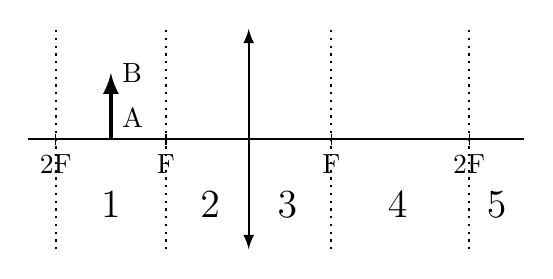
\begin{tikzpicture}[>=latex,scale=0.7]
    \draw (-4,0) -- (5,0); \draw[thick, <->] (0,-2) -- (0,2);
    \foreach \x/\l in {-3.5/2F, -1.5/F, 1.5/F, 4/2F} {
        \draw (\x,0.1) -- (\x,-0.1) node[below] {\l};
        \draw[dotted, thick] (\x,-2) -- (\x,2);
    }
    \draw[ultra thick, ->] (-2.5,0) node[above right] {A} -- (-2.5,1.2) node[right] {B};
    \foreach \x/\n in {-2.5/1, -0.7/2, 0.7/3, 2.7/4, 4.5/5} \node at (\x, -1.2) {\Large \n};
\end{tikzpicture}

\begin{enumerate}[label=\Alph*)]
\item 5
\item 4
\item 3
\item 2
\end{enumerate}

\item AB buyumning yig‘uvchi linzadagi tasviri qanday bo‘ladi?

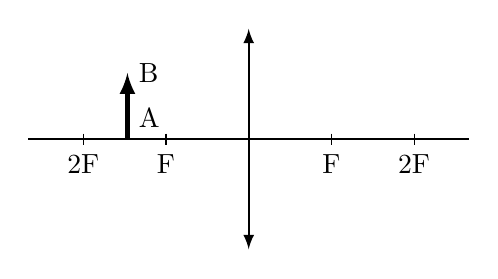
\begin{tikzpicture}[>=latex,scale=0.7]
    \draw (-4,0) -- (4,0); \draw[thick, <->] (0,-2) -- (0,2);
    \foreach \x/\l in {-3/2F, -1.5/F, 1.5/F, 3/2F} {\draw (\x,0.1) -- (\x,-0.1) node[below] {\l};}
    \draw[ultra thick, ->] (-2.2,0) node[above right] {A} -- (-2.2,1.2) node[right] {B};
\end{tikzpicture}

\begin{enumerate}[label=\Alph*)]
\item mavhum, to‘g‘ri, kichraygan.
\item mavhum, teskari, kattalashgan.
\item haqiqiy, teskari, kattalashgan.
\item haqiqiy, to‘g‘ri, kichraygan.
\end{enumerate}

\item Rasmda OO$'$ — linzaning bosh optik o‘qi, $S$ — buyum, $S'$ — uning haqiqiy tasviri. Bu qanday linza va nima yaqinroq joylashgan: buyumgami yoki uning tasvirigami?

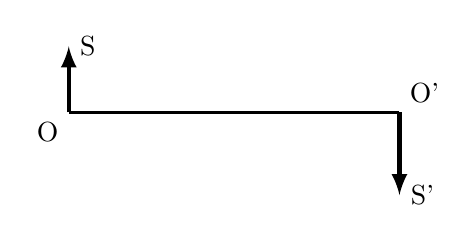
\begin{tikzpicture}[>=latex,scale=0.7]
    \draw[thick] (0,0) node[below left] {O} -- (6,0) node[above right] {O'};
    \draw[ultra thick, ->] (0,0) -- (0,1.2) node[right] {S};
    \draw[ultra thick, ->] (6,0) -- (6,-1.5) node[right] {S'};
\end{tikzpicture}

\begin{enumerate}[label=\Alph*)]
\item sochuvchi, $S'$ ga.
\item sochuvchi, $S$ ga.
\item yig‘uvchi, $S'$ ga.
\item yig‘uvchi, $S$ ga.
\item yig‘uvchi, $S$ va $S'$ dan bir xil masofada.
\end{enumerate}

\item Buyum yupqa yig‘uvchi linzadan $F<d<2F$ tengsizlikni qanoatlantiruvchi $d$ masofada joylashgan bo‘lsa, uning tasviri qanday bo‘ladi?

\begin{enumerate}[label=\Alph*)]
\item mavhum va kichiklashgan, to‘g‘ri.
\item mavhum va kattalashgan, to‘g‘ri.
\item mavhum va kichiklashgan, teskari.
\item haqiqiy va kichiklashgan, teskari.
\item haqiqiy va kattalashgan, teskari.
\end{enumerate}

\item Jism yig‘uvchi linzadan ikkilangan fokus masofadan ortiqroq masofada joylashgan. Uning linzadagi tasviri

\begin{enumerate}[label=\Alph*)]
\item mavhum va kattalashgan.
\item mavhum va kichiklashgan.
\item mavhum va teskari.
\item haqiqiy va kichiklashgan.
\item haqiqiy va kattalashgan.
\end{enumerate}

\item Buyum linzadan uning ikkilangan fokus masofasidan uzoqroqda joylashganida tasvir hosil bo‘ladi?

\begin{enumerate}[label=\Alph*)]
\item haqiqiy, kichraygan.
\item haqiqiy, kattalashgan.
\item haqiqiy, teng.
\item mavhum, kattalashgan.
\item TJY.
\end{enumerate}

\item Buyum yupqa yig‘uvchi linzadan $d>2F$ masofada joylashtirilgan bo‘lsa, uning tasviri qanday bo‘ladi?

\begin{enumerate}[label=\Alph*)]
\item mavhum va kattalashgan, to‘g‘ri.
\item mavhum va kichiklashgan, teskari.
\item haqiqiy va kichiklashgan, teskari.
\item haqiqiy va kattalashgan, teskari.
\end{enumerate}

\item Linza yordamida buyumning kichik teskari tasviri hosil qilindi. Bu qanday linza va qayerda joylashgan?

\begin{enumerate}[label=\Alph*)]
\item botiq; linzadan ixtiyoriy masofada.
\item botiq; linzaning ikkilangan fokus masofasidan uzoqda.
\item qavariq; fokus bilan ikkilangan fokus oralig‘ida.
\item qavariq; linzaning ikkilangan fokus masofasidan uzoqda.
\end{enumerate}

\item Yig‘uvchi linzadan buyumgacha qanday masofada tasvir haqiqiy, to‘nkarilgan va kichiklashgan bo‘ladi?

\begin{enumerate}[label=\Alph*)]
\item $d=2F$
\item $d>2F$
\item $d<2F$
\item $d<F$
\end{enumerate}

\item Rasmda linzaning vaziyati, bosh optik o‘qi, fokuslari va MN buyum ko‘rsatilgan. Buyumning linza hosil qiladigan tasviri qaysi sohada joylashadi?

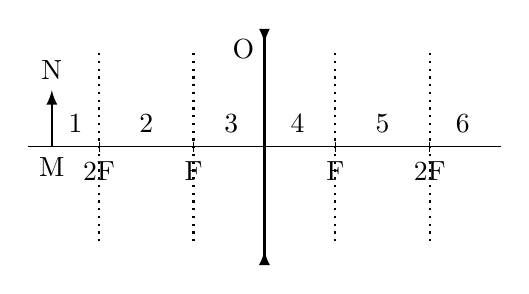
\begin{tikzpicture}[>=latex,scale=0.6]
    \draw (-5,0) -- (5,0); \draw[thick, >-<] (0,-2.5) -- (0,2.5) node[below left] {O};
    \foreach \x/\l in {-3.5/2F, -1.5/F, 1.5/F, 3.5/2F} {
        \draw (\x,0.1) -- (\x,-0.1) node[below] {\l};
        \draw[dotted, thick] (\x,-2) -- (\x,2);
    }
    \draw[thick, ->] (-4.5,0) node[below] {M} -- (-4.5,1.2) node[above] {N};
    \foreach \x/\n in {-4/1, -2.5/2, -0.7/3, 0.7/4, 2.5/5, 4.2/6} \node at (\x, 0.5) {\n};
\end{tikzpicture}

\begin{enumerate}[label=\Alph*)]
\item 2
\item 6
\item 5
\item 3
\end{enumerate}

\item Rasmda linza, buyum, linzaning bosh optik o‘qi va fokuslari tasvirlangan. Shu vaziyatdagi buyumning tasviri qanday bo‘ladi?

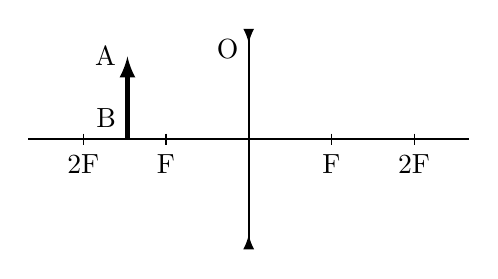
\begin{tikzpicture}[>=latex,scale=0.7]
    \draw (-4,0) -- (4,0); \draw[thick, >-<] (0,-2) -- (0,2) node[below left] {O};
    \foreach \x/\l in {-3/2F, -1.5/F, 1.5/F, 3/2F} {\draw (\x,0.1) -- (\x,-0.1) node[below] {\l};}
    \draw[ultra thick, ->] (-2.2,0) node[above left] {B} -- (-2.2,1.5) node[left] {A};
\end{tikzpicture}

\begin{enumerate}[label=\Alph*)]
\item mavhum va kichiklashgan.
\item haqiqiy va kattalashgan.
\item haqiqiy va kichiklashgan.
\item mavhum va kattalashgan.
\end{enumerate}

\item Chizmada keltirilgan buyumning sochuvchi linzadagi tasviri qanday bo‘ladi?

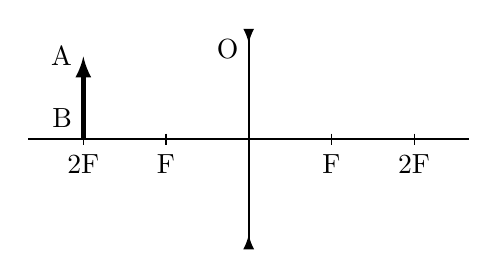
\begin{tikzpicture}[>=latex, scale=0.7]
    \draw (-4,0) -- (4,0); \draw[thick, >-<] (0,-2) -- (0,2) node[below left] {O};
    \foreach \x/\l in {-3/2F, -1.5/F, 1.5/F, 3/2F} {\draw (\x,0.1) -- (\x,-0.1) node[below] {\l};}
    \draw[ultra thick, ->] (-3,0) node[above left] {B} -- (-3,1.5) node[left] {A};
\end{tikzpicture}

\begin{enumerate}[label=\Alph*)]
\item mavhum, to‘g‘ri, kattalashgan.
\item haqiqiy, teskari, kichraygan.
\item haqiqiy, teskari, kattalashgan.
\item mavhum, to‘g‘ri, kichraygan.
\end{enumerate}

\item Rasmda OO$'$ — linzaning bosh optik o‘qi, $S$ — buyum, $S'$ — uning mavhum tasviri. Bu qanday linza va tasvir qaysi tomonda joylashgan?

\begin{tikzpicture}[>=latex,scale=0.6]
    \draw[thick] (0,0) node[left] {O} -- (8,0) node[right] {O'};
    \draw[thick, ->] (1,0) -- (1,2) node[right] {S};
    \draw[thick, dashed, ->] (4,0) -- (4,1) node[right] {S'};
\end{tikzpicture}

\begin{enumerate}[label=\Alph*)]
\item yig‘uvchi, $S'$ dan chap tomonda.
\item sochuvchi, $S'$ dan chap tomonda.
\item yig‘uvchi, $S'$ dan o‘ng tomonda.
\item sochuvchi, $S'$ dan o‘ng tomonda.
\item sochuvchi, $S$ va $S'$ orasida.
\end{enumerate}

\item Agar buyum yupqa sochuvchi linzadan uning ikkilangan fokus masofasiga nisbatan uzoqroq joylashgan bo‘lsa, uning tasviri qanday bo‘ladi?

\begin{enumerate}[label=\Alph*)]
\item to‘nkarilgan, haqiqiy, natural kattalikda.
\item kichiklashgan, to‘g‘ri, mavhum.
\item kattalashgan, to‘nkarilgan, haqiqiy.
\item to‘g‘ri, haqiqiy, natural kattalikda.
\item kichiklashgan, to‘nkarilgan, haqiqiy.
\end{enumerate}

\item Sochuvchi linza yordamida buyumning haqiqiy tasvirini olish mumkinmi? Agar mumkin bo‘lsa, buyumni qayerga joylashtirish kerak?

\begin{enumerate}[label=\Alph*)]
\item ha, $2F$ ga.
\item ha, $F$ va $2F$ orasiga.
\item yo‘q, mumkin emas.
\item ha, $2F$ dan uzoqqa.
\item ha, linza bilan uning fokusi orasiga.
\end{enumerate}

\item Buyum yupqa yig‘uvchi linzadan $2F$ masofada joylashgan bo‘lsa, uning tasviri qanday bo‘ladi?

\begin{enumerate}[label=\Alph*)]
\item to‘g‘ri, mavhum, kichiklashgan.
\item teskari, haqiqiy, o‘zining kattaligida.
\item teskari, haqiqiy, kattalashgan.
\item to‘g‘ri, haqiqiy, o‘zining kattaligida.
\item teskari, haqiqiy, kichiklashgan.
\end{enumerate}

\item Optik sistema fokus masofasi 30 cm bo‘lgan uchta yig‘uvchi linzadan iborat. Linzalar markazlari orasidagi masofa ham 30 cm ga teng. Buyum chap tomondagi linzadan 60 cm uzoqlikda joylashgan. Buyumning tasviri qayerda va qanday bo‘ladi?

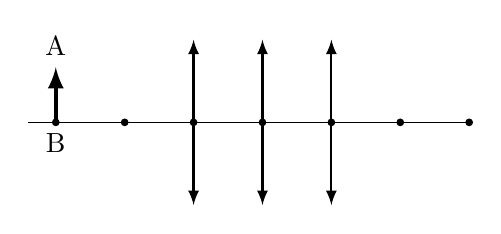
\begin{tikzpicture}[>=latex,scale=0.7]
    \draw (0,0) -- (8,0);
    \foreach \x in {0.5, 1.75, 3, 4.25, 5.5, 6.75, 8} \fill (\x,0) circle (2pt);
    \draw[ultra thick, ->] (0.5,0) node[below] {B} -- (0.5,1) node[above] {A};
    \foreach \x in {3, 4.25, 5.5} \draw[thick, <->] (\x, -1.5) -- (\x, 1.5);
\end{tikzpicture}

\begin{enumerate}[label=\Alph*)]
\item chap tomondagi linza o‘rnida, haqiqiy.
\item o‘rtadagi linza o‘rnida, haqiqiy.
\item o‘ng tomondagi linzadan 60 cm uzoqlikda, haqiqiy.
\item o‘rtadagi linza o‘rnida, mavhum.
\item o‘ng tomondagi linzadan 60 cm uzoqlikda, mavhum.
\end{enumerate}

\end{enumerate}



\begin{center}
\begin{tabular}{|c|c|c|c|c|c|c|c|c|c|}
\hline
1e & 2e & 3b & 4b & 5a & 6a & 7d & 8d & 9e & 10d \\
\hline
11a & 12d & 13e & 14c & 15e & 16a & 17e & 18c & 19b & 20c \\
\hline
21b & 22d & & & & & & & & \\
\hline
\end{tabular}
\end{center}













\section{Linza formulasi}
\begin{enumerate}

\item Yig‘uvchi linzadan buyumgacha bo‘lgan masofa 1 m, tasvirdan linzagacha 25 cm. Linzaning fokus masofasi necha cm?
\begin{enumerate}[label=\Alph*)]
\item 20.
\item 15.
\item 12,5.
\item 33.
\item TJY.
\end{enumerate}

\item Buyum fokus masofasi 12 cm bo‘lgan linzadan 16 cm uzoqlikda qo‘yildi. Linzaning kattalashtirishi qanday?
\begin{enumerate}[label=\Alph*)]
\item 6.
\item 5.
\item 4.
\item 3.
\item 2.
\end{enumerate}

\item Yig‘uvchi linzaning fokus masofasi $F$ ga teng. Linzaning kattalashtirishi 2 ga teng bo‘lishi uchun buyum undan qanday masofada qo‘yilishi kerak?
\begin{enumerate}[label=\Alph*)]
\item $1{,}5F$.
\item $F$.
\item $2F$.
\item $3F$.
\item $4F$.
\end{enumerate}

\item Buyum fokus masofasi 50 cm bo‘lgan yig‘uvchi linzadan necha cm masofaga joylashtirilganda, 4 marta kattalashgan tasvir hosil qilishi mumkin?
\begin{enumerate}[label=\Alph*)]
\item 25.
\item 31,2.
\item 50.
\item 62,5.
\item 75.
\end{enumerate}

\item Fokus masofasi $F$ bo‘lgan yig‘uvchi linza yordamida ekranda tasvir hosil qilish uchun buyum va ekran orasidagi masofa kamida qanday bo‘lishi kerak?
\begin{enumerate}[label=\Alph*)]
\item $5F$.
\item $4F$.
\item $3F$.
\item $2F$.
\item $F$.
\end{enumerate}

\item Fokus masofasi 1 m bo‘lgan yig‘uvchi linzadan necha metr masofaga buyumni joylashtirsak, uning mavhum tasviri linzadan 3 masofada hosil bo‘ladi?
\begin{enumerate}[label=\Alph*)]
\item 2.
\item 1,5.
\item 1,25.
\item 1.
\item 0,75.
\end{enumerate}

\item Fokus masofasi 36 cm bo‘lgan linzadan 18 cm uzoqlikda joylashgan buyumning kattalashgan mavhum tasviri linzadan necha cm masofada hosil bo‘ladi?
\begin{enumerate}[label=\Alph*)]
\item 36.
\item 18.
\item 12.
\item 9.
\item 6.
\end{enumerate}

\item Buyumni linzadan 25 cm masofaga qo‘ysak, uning haqiqiy tasviri linzadan 50 cm narida hosil bo‘ladi. Buyum shu linzadan 0,2 m masofaga qo‘yilsa, tasvir linzadan necha cm masofada hosil bo‘ladi?
\begin{enumerate}[label=\Alph*)]
\item 40.
\item 20.
\item 25.
\item 100.
\item 35.
\end{enumerate}

\item Yig‘uvchi linzadan buyumgacha bo‘lgan masofa 0,5 m va tasvirdan linzagacha bo‘lgan masofa 1 m bo‘lsa, linzaning fokus masofasi qanday (m)?
\begin{enumerate}[label=\Alph*)]
\item 1,5.
\item 0,33.
\item 5.
\item 3.
\item TJY.
\end{enumerate}

\item Buyumni fokus masofasi $F$ bo‘lgan yig‘uvchi linzadan qanday masofaga qo‘yganda, uning tasviri o‘ziga teng bo‘ladi?
\begin{enumerate}[label=\Alph*)]
\item $F$.
\item $2F$.
\item $3F$.
\item $4F$.
\item $F/2$.
\end{enumerate}

\item Buyum bilan haqiqiy tasvir orasidagi masofaning eng kichik qiymatini toping. Linzaning fokus masofasi $F$ ga teng.
\begin{enumerate}[label=\Alph*)]
\item $F$.
\item $3F$.
\item $2F$.
\item $4F$.
\item $5F$.
\end{enumerate}

\item Fokus masofasi 5 cm bo‘lgan linza yordamida buyumning mavhum tasviri linzadan 10 cm masofada hosil qilindi. Linzaning kattalashtirishini toping.
\begin{enumerate}[label=\Alph*)]
\item 10.
\item 6.
\item 5.
\item 3.
\item 2.
\end{enumerate}

\item Buyum va uning tasviri orasidagi masofa eng kichik bo‘lishi uchun buyumni yig‘uvchi linzadan qanday masofada qo‘yish kerak?
\begin{enumerate}[label=\Alph*)]
\item $0{,}5F$.
\item $F$.
\item $F<d<2F$.
\item $2F$.
\item $d>2F$.
\end{enumerate}

\item Buyumdan linzagacha bo‘lgan masofa $d$ ga va linzaning fokus masofasi $F$ ga teng bo‘lsa, uning kattalashtirishi qanday bo‘ladi?
\begin{enumerate}[label=\Alph*)]
\item $\dfrac{d-F}{F}$.
\item $\dfrac{d}{d-F}$.
\item $\dfrac{F}{d-F}$.
\item $\dfrac{F-d}{F+d}$.
\item $\dfrac{F+d}{F-d}$.
\end{enumerate}

\item Linzaning fokus masofasi $F$, linzadan buyumgacha masofa $d$ bo‘lsa, linzaning kattalashtirishi qanday? (Tasvir haqiqiy)
\begin{enumerate}[label=\Alph*)]
\item $\dfrac{d-F}{Fd}$.
\item $\dfrac{dF}{d-F}$.
\item $\dfrac{d}{d-F}$.
\item $\dfrac{F}{d-F}$.
\item $\dfrac{d-F}{d+F}$.
\end{enumerate}




\item Fokus masofasi $F$ bo‘lgan yig‘uvchi linzada o‘lchami $a$ ga teng bo‘lgan buyumning haqiqiy tasviri hosil qilindi. Agar linzadan tasvirgacha bo‘lgan masofa $b$ bo‘lsa, tasvirning o‘lchami qanday?
\begin{enumerate}[label=\Alph*)]
\item $\dfrac{F}{a(f-F)}$.
\item $\dfrac{aF}{f-F}$.
\item $\dfrac{a(f-F)}{F}$.
\item $\dfrac{a(f+F)}{F}$.
\item $\dfrac{f-F}{aF}$.
\end{enumerate}

\item Yig‘uvchi linzada hosil bo‘lgan va $k$ marta kattalashgan tasvirda buyumgacha bo‘lgan masofa $L$ ga teng bo‘lsa, linzadan tasvirgacha bo‘lgan masofa nimaga teng bo‘ladi?
\begin{enumerate}[label=\Alph*)]
\item $k(k^2+1)L$.
\item $k(k+1)L$.
\item $\dfrac{k^2}{k+1}L$.
\item $\dfrac{k+1}{k}L$.
\item $\dfrac{k}{k+1}L$.
\end{enumerate}

\item Fokus masofasi $F$ ga teng. Linzaning kattalashtirishi 2 dan, ammo 3 dan kichik bo‘lishi uchun buyumni undan qanday uzoqlikda qo‘yish kerak?
\begin{enumerate}[label=\Alph*)]
\item $5F/3>d>3F/2$.
\item $3F<d<2F$.
\item $3F>d>2F$.
\item $4F/3<d<3F/2$.
\item TJY.
\end{enumerate}

\item Buyum yig‘uvchi linzaning fokusigacha bo‘lgan masofa 2 cm, haqiqiy tasvirdan ikkinchi fokusgacha bo‘lgan masofa 8 cm. Linzaning fokus masofasini aniqlang (cm).
\begin{enumerate}[label=\Alph*)]
\item 2,5.
\item 5.
\item 10.
\item 20.
\item 4.
\end{enumerate}

\item Yupqa linza fokusidan buyumgacha bo‘lgan $a$ masofa bilan ikkinchi fokusdan haqiqiy tasvirgacha bo‘lgan $b$ masofa ko‘paytmasi $(ab)$ ni linzaning fokus masofasi $F$ orqali ifodalang.
\begin{enumerate}[label=\Alph*)]
\item $2F^2/3$.
\item $2F^2$.
\item $F^3/(F+1)$.
\item $F^2/2$.
\item $F^2$.
\end{enumerate}

\item Yig‘uvchi linza yordamida yorug‘ nuqtaning tasviri hosil qilindi. Bunda linzadan nuqtagacha bo‘lgan masofa 50 cm, linzadan tasvirgacha masofa 12,5 cm. Linzaning fokus masofasi qanday (cm)?
\begin{enumerate}[label=\Alph*)]
\item 1.
\item 62,5.
\item 37,5.
\item 25.
\item 10.
\end{enumerate}

\item Buyumdan linzagacha bo‘lgan masofa 15 cm bo‘lganda, linzaning kattalashtirishi 2 ga teng bo‘lsa, linzaning fokus masofasi qanday (cm).
\begin{enumerate}[label=\Alph*)]
\item 7,5.
\item $2/3$.
\item 30.
\item 15.
\item 10.
\end{enumerate}

\item Linzadan 25 cm masofada joylashgan buyumning ekranda 4 marta kattalashgan tasviri hosil bo‘ladi. Linzaning fokus masofasini aniqlang (m).
\begin{enumerate}[label=\Alph*)]
\item 0,15.
\item 0,2.
\item 0,25.
\item 0,3.
\item 0,4.
\end{enumerate}

\item Buyum bilan tasvir orasidagi masofa 1,5 m va tasvir buyumdan 4 marta katta bo‘lsa, linzaning fokus masofasi qanday (cm)?
\begin{enumerate}[label=\Alph*)]
\item 24.
\item 18.
\item 22.
\item 6.
\item 26.
\end{enumerate}

\item Yig‘uvchi linza buyumning 8 marta kichiklashgan tasvirini hosil qilmoqda. Agar buyumdan linzagacha bo‘lgan masofa 10 cm ga qisqartirilsa, buyumning 4 marta kichiklashgan tasviri hosil bo‘ladi. Linzaning fokus masofasi necha cm?
\begin{enumerate}[label=\Alph*)]
\item 8.
\item 5.
\item 2,5.
\item 2.
\item 1,25.
\end{enumerate}

\item Buyumdan linzagacha masofa $d$ ga, kattalashtirish $k$ ga teng va tasvir mavhum bo‘lsa, linzaning fokus masofasi qanday?
\begin{enumerate}[label=\Alph*)]
\item $k^2(k+1)d$.
\item $\dfrac{k}{k+1}d$.
\item $\dfrac{k}{k-1}d$.
\item $\dfrac{k-1}{k}d$.
\item $\dfrac{k+1}{k}d$.
\end{enumerate}

\item Fokus masofasi 0,5 m ga teng bo‘lgan linza yordamida 5 marta kattalashtirilgan haqiqiy tasvir hosil qilish uchun buyumni linzadan necha metr masofaga qo‘yish kerak?
\begin{enumerate}[label=\Alph*)]
\item 0,4.
\item 0,6.
\item 1.
\item 1,24.
\item 1,6.
\end{enumerate}

\item Buyum bilan uning yig‘uvchi linzadagi haqiqiy tasviri orasidagi masofa 2,5 m. Linzadan tasvirgacha bo‘lgan masofa esa 2 m bo‘lsa, linzaning kattalashtirish koeffitsienti qanday?
\begin{enumerate}[label=\Alph*)]
\item 0,8.
\item 1,25.
\item 5.
\item 4.
\item 10.
\end{enumerate}

\item Ushbu rasmdagi $h$ o‘lchamli buyumning tasviri qanday o‘lchamga ega? ($h'-?$).
\begin{enumerate}[label=\Alph*)]
\item $h/3$.
\item $h$.
\item $2h$.
\item $3h/2$.
\item $3h$.
\end{enumerate}

\item Fokus masofasi 15 cm bo‘lgan yupqa yig‘uvchi linza yordamida buyumning 3 marta kattalashgan mavhum tasviri hosil qilindi. Buyumdan tasvirgacha bo‘lgan masofani (cm) aniqlang.
\begin{enumerate}[label=\Alph*)]
\item 20.
\item 10.
\item 30.
\item 40.
\item 15.
\end{enumerate}

\item Buyum bilan yig‘uvchi linza oralig‘i $3F$. Linzaning fokus masofasi $F$ bo‘lsa, tasvirning o‘lchami buyum o‘lchamidan necha marta katta bo‘ladi?
\begin{enumerate}[label=\Alph*)]
\item 3.
\item 2.
\item 4.
\item 5.
\item 2,5.
\end{enumerate}






\item Fokus masofasi 1 m bo‘lgan qavariq linzadan 3 m masofada jism turibdi. Linzaning chiziqli kattalashtirishini aniqlang.
\begin{enumerate}[label=\Alph*)]
\item 1.
\item 1,5.
\item 2.
\item 3.
\item 0,5.
\end{enumerate}

\item Yig‘uvchi linzadan buyumgacha bo‘lgan masofa fokus masofadan uch marta katta bo‘lsa, kattalashtirish koeffitsienti qanday?
\begin{enumerate}[label=\Alph*)]
\item 3.
\item 2.
\item 1,5.
\item 0,75.
\item 0,5.
\end{enumerate}

\item Buyum linzadan $4F$ masofada joylashgan. Shu buyumning ekrandagi tasviri o‘zidan necha marta kichik bo‘ladi?
\begin{enumerate}[label=\Alph*)]
\item 2.
\item 3.
\item 4.
\item 5.
\item 8.
\end{enumerate}

\item Agar haqiqiy tasvir buyumdan 3 marta kichik bo‘lsa, buyum linzadan qanday masofada joylashgan? Linzaning fokus masofasi $F$.
\begin{enumerate}[label=\Alph*)]
\item $4/3F$.
\item $1{,}5F$.
\item $2F$.
\item $4F$.
\item $6F$.
\end{enumerate}

\item Uzunligi 1 cm bo‘lgan igna fokus masofasi 3 cm bo‘lgan linzaning bosh optik o‘qiga o‘q bo‘ylab joylashtirildi. Agar ignaning bir uchi linza fokusidan 1 cm masofada yotgan bo‘lsa, ignaning haqiqiy tasviridagi uzunligini aniqlang (cm).
\begin{enumerate}[label=\Alph*)]
\item 1,5.
\item 2,5.
\item 3,5.
\item 4,5.
\item 5,5.
\end{enumerate}

\item Yig‘uvchi linzadan buyumgacha bo‘lgan masofa $d$ va linzaning fokus masofasi $F$ qanday munosabatda bo‘lganda, linzaning kattalashtirishi 0,5 ga teng bo‘ladi?
\begin{enumerate}[label=\Alph*)]
\item $d=4F$.
\item $d=2F$.
\item $d=F$.
\item $d=3F$.
\item $d=F/2$.
\end{enumerate}

\item Buyum yig‘uvchi linzadan $d=nF$ masofada joylashgan bo‘lsa, linza bilan tasvir orasidagi masofa qanday bo‘ladi?
\begin{enumerate}[label=\Alph*)]
\item $\dfrac{nF}{n-1}$.
\item $\dfrac{F(n+1)}{n}$.
\item $\dfrac{F}{n}$.
\item $\dfrac{F}{n+1}$.
\item $\dfrac{F(n-1)}{n}$.
\end{enumerate}

\item Qo‘zg‘almas buyum va ekran orasida linza surilmoqda. Linzaning ikki holatida ekranda buyumning $h_1$ va $h_2$ o‘lchamlari aniqlangan. Buyumning o‘lchami qanday?
\begin{enumerate}[label=\Alph*)]
\item $\sqrt{2h_1h_2}$.
\item $\sqrt{h_1h_2}$.
\item $\dfrac{h_1-h_2}{2}$.
\item $\dfrac{2h_1h_2}{h_1+h_2}$.
\item $\dfrac{h_1+h_2}{2}$.
\end{enumerate}

\item Sochuvchi yupqa linza formulasi qaysi javobda berilgan?
\begin{enumerate}[label=\Alph*)]
\item $-\dfrac1F=\dfrac1d-\dfrac1{f'}$.
\item $\dfrac1F=\dfrac1d-\dfrac1{f'}$.
\item $\dfrac1F=\dfrac1d+\dfrac1{f'}$.
\item $-\dfrac1F=\dfrac1d-\dfrac1d'$.
\item $-\dfrac1F=\dfrac1d+\dfrac1{f'}$.
\end{enumerate}

\item Shu’lalanayotgan nuqta fokus masofasi 10 cm bo‘lgan sochuvchi linza fokusida turibdi. Uning tasviri linzadan qanday masofada hosil bo‘ladi?
\begin{enumerate}[label=\Alph*)]
\item 10 cm.
\item 20 cm.
\item 5 cm.
\item cheksizlikda.
\item tasvir hosil bo‘lmaydi.
\end{enumerate}

\item Nuqtaviy yorug‘lik manbai fokus masofasi $F$ bo‘lgan sochuvchi linzaning fokusida turibdi. Uning tasviri linzadan qanday masofada hosil bo‘ladi?
\begin{enumerate}[label=\Alph*)]
\item $F/4$.
\item $F/2$.
\item $F$.
\item $1{,}5F$.
\item $2F$.
\end{enumerate}

\item Buyumning sochuvchi linza berayotgan haqiqiy tasviri o‘zidan 2 marta kichik bo‘lishi uchun, buyumni linzadan qanday masofada joylashtirish kerak? ($F$–linzaning fokus masofasi).
\begin{enumerate}[label=\Alph*)]
\item $F/2$.
\item bu mumkin emas.
\item $2F$.
\item $F$.
\item $3F/2$.
\end{enumerate}

\item Fokus masofasi 24 cm bo‘lgan linzadan 12 cm masofada joylashgan buyumning kichiklashgan mavhum tasviri linzadan necha cm masofada hosil bo‘ladi?
\begin{enumerate}[label=\Alph*)]
\item 4.
\item 8.
\item 12.
\item 18.
\item 24.
\end{enumerate}

\item Fokus masofasi 15 cm bo‘lgan linzadan 10 cm masofada joylashgan buyumning kichiklashgan tasviri linzadan qanday masofada hosil bo‘ladi? (cm)
\begin{enumerate}[label=\Alph*)]
\item 6.
\item 7,5.
\item 16.
\item 25.
\item 30.
\end{enumerate}

\item Fokus masofasi 10 cm bo‘lgan linzadan 15 cm masofada joylashgan buyumning mavhum tasviri linzadan necha cm masofada hosil bo‘ladi?
\begin{enumerate}[label=\Alph*)]
\item 6.
\item 7,5.
\item 16.
\item 20.
\item 30.
\end{enumerate}

\item Fokus masofasi 20 cm bo‘lgan linzadan 15 cm uzoqlikda buyumning kichiklashgan mavhum tasviri hosil bo‘ldi. Buyum linzadan necha cm masofada joylashgan?
\begin{enumerate}[label=\Alph*)]
\item 8,6.
\item 17,2.
\item 30.
\item 60.
\item 75.
\end{enumerate}

\item Buyum sochuvchi linza oldida undan $2F$ masofada turibdi. Tasvir linzadan qanday masofada hosil bo‘ladi?
\begin{enumerate}[label=\Alph*)]
\item $0{,}5F$.
\item $F$.
\item $F/3$.
\item $4F/3$.
\item $2F/3$.
\end{enumerate}

\item Buyumdan sochuvchi linzagacha bo‘lgan masofa linzaning fokus masofasidan $n$ marta katta bo‘lsa, tasvir buyumdan necha marta kichik bo‘ladi?
\begin{enumerate}[label=\Alph*)]
\item $n+1$.
\item $n$.
\item $n-1$.
\item $\dfrac1{n+1}$.
\item $\dfrac1{n-1}$.
\end{enumerate}

\item Agar buyumdan sochuvchi linzagacha bo‘lgan masofa linzaning fokus masofasidan $m$ marta katta bo‘lsa, tasvir buyumdan necha marta kichik bo‘ladi?
\begin{enumerate}[label=\Alph*)]
\item $m-1$.
\item $m+1$.
\item $\dfrac{m}{m+1}$.
\item $\dfrac{m}{m-1}$.
\item $\dfrac{m-1}{m+1}$.
\end{enumerate}

\item Linzaning optik kuchi birligi – dioptriyani boshqa birliklar orqali qanday ifodalash mumkin?
\begin{enumerate}[label=\Alph*)]
\item cm$^{-1}$.
\item m.
\item m$^{-1}$.
\item N$^{-1}$.
\item TJY.
\end{enumerate}

\item Linzaning fokus masofasi 4 cm. Uning optik kuchi necha dioptriya?
\begin{enumerate}[label=\Alph*)]
\item 4.
\item 0,4.
\item 0,25.
\item 25.
\item TJY.
\end{enumerate}

\item Fokus masofasi 12,5 cm bo‘lgan linzaning optik kuchi necha dioptriya?
\begin{enumerate}[label=\Alph*)]
\item 4.
\item 2.
\item 8.
\item 12,5.
\item 0,8.
\end{enumerate}

\item Fokus masofasi 5 cm bo‘lgan sochuvchi linzaning optik kuchini aniqlang (dioptriyalarda).
\begin{enumerate}[label=\Alph*)]
\item 5.
\item $-0{,}2$.
\item 0,05.
\item $-20$.
\item TJY.
\end{enumerate}

\item Linzaning optik kuchi 4 D. Shu linzaning fokus masofasi necha cm?
\begin{enumerate}[label=\Alph*)]
\item 0,25.
\item 25.
\item 4.
\item 40.
\item TJY.
\end{enumerate}

\item Rasmda ko‘rsatilgan linzalar sistemasining optik kuchini aniqlang (D).
\begin{enumerate}[label=\Alph*)]
\item $-1{,}5$.
\item 7.
\item $-3$.
\item 3,5.
\item TJY.
\end{enumerate}

\item Fokus masofalari 20 va 30 cm bo‘lgan ikkita yupqa linzani birlashtirsak, hosil bo‘lgan linzaning fokus masofasi qanday bo‘ladi? (cm)
\begin{enumerate}[label=\Alph*)]
\item 56.
\item 50.
\item 34.
\item 12.
\item 10.
\end{enumerate}





\item Ikkita linza umumiy bosh optik o‘qqa ega. 1-linzaning fokus masofasi $F_1=-0{,}125$ m, 2-linzaning optik kuchi $D_2=8$ D. Linzalar sistemasining optik kuchini toping (D).
\begin{enumerate}[label=\Alph*)]
\item 0.
\item 2.
\item 4.
\item 8.
\item $-2$.
\end{enumerate}

\item Optik kuchi 12 D bo‘lgan yig‘uvchi linzadan 50 cm masofada joylashgan buyumning tasviri linzadan necha cm masofada hosil bo‘ladi?
\begin{enumerate}[label=\Alph*)]
\item 60.
\item 25.
\item 12.
\item 10.
\item 6.
\end{enumerate}

\item Optik kuchi 2 D bo‘lgan linzada buyumning 5 marta kattalashgan haqiqiy tasvirini hosil qilayotgan bo‘lsa, linzadan tasvirgacha bo‘lgan masofa necha metr?
\begin{enumerate}[label=\Alph*)]
\item 2.
\item 1,5.
\item 3.
\item 0,5.
\item 1.
\end{enumerate}

\item Optik kuchi 3 D bo‘lgan linzada buyumning 5 marta kattalashgan haqiqiy tasviri hosil bo‘ldi. Buyumdan linzagacha necha metr?
\begin{enumerate}[label=\Alph*)]
\item 0,3.
\item 0,8.
\item 0,6.
\item 0,5.
\item 0,4.
\end{enumerate}

\item Jism optik kuchi 10 D bo‘lgan qavariq linzadan 30 cm masofada turibdi. Linzaning kattalashtirishini toping.
\begin{enumerate}[label=\Alph*)]
\item 1,5.
\item 1.
\item 0,8.
\item 0,5.
\item 2.
\end{enumerate}

\item Buyumning 5 marta kattalashgan tasvirini hosil qilish uchun optik kuchi qanday linza kerak va uni buyumdan qanday masofaga qo‘yish kerak? Buyumdan ekrangacha masofa 3 m.
\begin{enumerate}[label=\Alph*)]
\item 2,6 D; 2 m.
\item 3 D; 1 m.
\item 2,4 D; 0,5 m.
\item 1 D; 1,5 m.
\item TJY.
\end{enumerate}

\item Buyumning to‘g‘ri tasviri hosil bo‘lishi uchun buyum optik kuchi 2 D bo‘lgan yig‘uvchi linzadan ko‘pi bilan necha metr masofada bo‘lishi kerak?
\begin{enumerate}[label=\Alph*)]
\item 0,4.
\item 0,5.
\item 0,8.
\item 2.
\item 4.
\end{enumerate}

\item Tasvir optik kuchi 3 D bo‘lgan linzadan 50 cm uzoqlikda, buyum turgan tomonda hosil bo‘ldi. Buyum linzadan necha metr masofada joylashgan?
\begin{enumerate}[label=\Alph*)]
\item 1.
\item 0,5.
\item 0,4.
\item 0,25.
\item 0,2.
\end{enumerate}

\item Optik kuchi $+7$ dptr bo‘lgan yig‘uvchi va $-2$ dptr bo‘lgan sochuvchi linzalar ketma-ket joylashgan bo‘lib, ularning optik o‘qlari to‘g‘ri chiziqda yotadi. Agar buyum linzalardan 22 cm uzoqlikda joylashgan bo‘lsa, linzalar sistemasining chiziqli kattalashtirishini toping.
\begin{enumerate}[label=\Alph*)]
\item 10.
\item 5.
\item 0,5.
\item 4.
\item 2.
\end{enumerate}

\item Buyum optik kuchi $-1$ D bo‘lgan sochuvchi linzadan 4 m uzoqlikda turibdi. Tasvir linzadan necha metr masofada hosil bo‘ladi?
\begin{enumerate}[label=\Alph*)]
\item 3.
\item 1,25.
\item 1,33.
\item 1.
\item 0,8.
\end{enumerate}

\item Optik kuchi $-4$ D bo‘lgan sochuvchi linzadan 1 m masofada joylashgan buyumning tasviri linzadan qanday masofada hosil bo‘ladi?
\begin{enumerate}[label=\Alph*)]
\item 20 cm.
\item 1 m.
\item 0,4 m.
\item 10 cm.
\item 1 cm.
\end{enumerate}

\item Tasvirning o‘lchamlari buyum o‘lchamidan 4 marta kichik bo‘lishi uchun buyum optik kuchi $-4$ D bo‘lgan sochuvchi linzadan necha metr masofaga joylashtirilishi kerak?
\begin{enumerate}[label=\Alph*)]
\item 0,75.
\item 0,25.
\item 1.
\item 0,5.
\item 0,85.
\end{enumerate}

\item Agar linzadan 10 cm uzoqlikda joylashtirilgan buyumning mavhum tasviri linzadan 20 cm uzoqlikda hosil bo‘lsa, linzaning optik kuchi qanday (D)?
\begin{enumerate}[label=\Alph*)]
\item $+10$.
\item $-20$.
\item $+20$.
\item $-5$.
\item $+5$.
\end{enumerate}

\item Buyumning mavhum tasviri linzadan 50 cm masofada hosil bo‘ldi. Agar buyumdan linzagacha bo‘lgan masofa 25 cm bo‘lsa, linzaning optik kuchi necha D ga teng?
\begin{enumerate}[label=\Alph*)]
\item 4.
\item $-2$.
\item 3.
\item 2.
\item 3,5.
\end{enumerate}

\item Agar linzadan 12,5 cm masofada joylashgan buyumning 2 marta kattalashgan mavhum tasviri hosil bo‘lsa, linzaning optik kuchi necha dioptriya?
\begin{enumerate}[label=\Alph*)]
\item 2.
\item $-2$.
\item 4.
\item $-4$.
\item 6.
\end{enumerate}

\item Linzadan 20 cm masofada joylashgan buyumning to‘g‘ri, kattalashgan tasviri buyumdan 30 cm masofada hosil bo‘ldi. Linzaning optik kuchini aniqlang (D).
\begin{enumerate}[label=\Alph*)]
\item $-5$.
\item 3.
\item $-3$.
\item 15.
\item 10.
\end{enumerate}

\item Tasvir optik kuchi 3 D bo‘lgan linzadan 50 cm uzoqlikda, buyum turgan tomonda hosil bo‘ldi. Buyum linzadan necha metr masofada joylashgan?
\begin{enumerate}[label=\Alph*)]
\item 1.
\item 0,5.
\item 0,4.
\item 0,25.
\item 0,2.
\end{enumerate}

\item Ekranda yig‘uvchi linzadan 1 m masofada joylashgan buyumning 2 marta kattalashgan tasviri ko‘rinayotgan bo‘lsa, linzaning optik kuchi necha dioptriya?
\begin{enumerate}[label=\Alph*)]
\item 4.
\item 3.
\item 2.
\item 0,5.
\item 1,5.
\end{enumerate}

\item Buyum bilan ekran orasidagi masofa 2 m. Agar linzaning kattalashtirishi 2 ga teng bo‘lsa, uning optik kuchi qanday (D)?
\begin{enumerate}[label=\Alph*)]
\item $+2{,}25$.
\item $+3{,}12$.
\item $+1{,}26$.
\item $-2{,}25$.
\item $-3{,}12$.
\end{enumerate}

\item Linzadan 10 cm masofada joylashgan buyumning 2 marta kichiklashgan mavhum tasviri hosil bo‘ldi. Linzaning optik kuchini aniqlang (D).
\begin{enumerate}[label=\Alph*)]
\item 5.
\item $-5$.
\item 10.
\item $-10$.
\item 30.
\end{enumerate}

\item Sochuvchi linzadan 1 m masofadagi buyumning tasviri linzadan 20 cm masofada joylashgan. Linzaning optik kuchini aniqlang (D).
\begin{enumerate}[label=\Alph*)]
\item $-6$.
\item 5.
\item 6.
\item $-4$.
\item $-3$.
\end{enumerate}

\item Sochuvchi linzadan 40 cm uzoqlikda buyumning 5 marta kichraygan mavhum tasviri hosil bo‘ldi. Linzaning optik kuchini aniqlang (D).
\begin{enumerate}[label=\Alph*)]
\item $-9$.
\item $-5$.
\item $-8$.
\item $-2$.
\item $-12$.
\end{enumerate}

\item Sochuvchi linzadan 50 cm uzoqlikdagi jismning mavhum tasviri 5 marta kichiklashgan holda hosil bo‘ldi. Shu linzaning optik kuchi necha D?
\begin{enumerate}[label=\Alph*)]
\item $-7$.
\item $-8$.
\item $-9$.
\item $-10$.
\item 8.
\end{enumerate}

\item Ikki tomoni qavariq va sirtlarining egrilik radiuslari bir xil $R_1=R_2=0{,}5$ m va sindirish ko‘rsatkichi 1,5 bo‘lgan shishadan yasalgan yig‘uvchi linzaning optik kuchi qanday (D)?
\begin{enumerate}[label=\Alph*)]
\item 2.
\item 0,5.
\item 1.
\item 1,5.
\item 2,5.
\end{enumerate}

\item Radiuslari 5 cm va 10 cm bo‘lgan ikki tomoni qavariq linzaning vakuumdagi fokus masofasi 10 cm ga teng. Linza materialining absolyut sindirish ko‘rsatkichini toping.
\begin{enumerate}[label=\Alph*)]
\item 2.
\item 1,5.
\item $4/3$.
\item 2,5.
\item 1,25.
\end{enumerate}


\item Radiuslari 10 cm va 15 cm bo‘lgan ikki tomonlama qavariq linzaning vakuumdagi fokus masofasini aniqlang (cm). Linza materialining absolyut sindirish ko‘rsatkichi 1,6 ga teng.
\begin{enumerate}[label=\Alph*)]
\item 20.
\item 15.
\item 40.
\item 25.
\item 10.
\end{enumerate}

\item Absolyut sindirish ko‘rsatkichi 1,5 bo‘lgan shishadan yasalgan botiq-qavariq linzaning bosh fokus masofasi 24 cm. Bu linzaning biri ikkinchisidan 2 marta kichik bo‘lgan egrilik radiusini toping (cm).
\begin{enumerate}[label=\Alph*)]
\item 14.
\item 16.
\item 18.
\item 15.
\item 12.
\end{enumerate}

\item Absolyut sindirish ko‘rsatkichi 1,6 bo‘lgan shishadan sirtining egrilik radiusi 18 cm ga teng bo‘lgan yassi-qavariq yupqa linza yasaldi. Linza yassi sirtiga tik ravishda tushayotgan parallel nurlar dastasi linzadan qanday masofada yig‘iladi? (cm)
\begin{enumerate}[label=\Alph*)]
\item 30.
\item 18.
\item 9.
\item 36.
\item 3.
\end{enumerate}

\item Optik kuchi 8 D bo‘lgan linza sindirish ko‘rsatkichi 1,5 bo‘lgan shishadan yasalgan. Linza suyuqlikka tushirilganda fokus masofasi 1 m bo‘lgan sochuvchi linzaga aylandi. Suyuqlikning sindirish ko‘rsatkichini aniqlang.
\begin{enumerate}[label=\Alph*)]
\item 1,6.
\item 2.
\item 1,4.
\item 1,7.
\item 1,8.
\end{enumerate}

\item Qavariq linzaning fokus masofasi va linza sirtlarining egrilik radiuslari bir-biriga teng bo‘lsa, linza materialining sindirish ko‘rsatkichi qanday?
\begin{enumerate}[label=\Alph*)]
\item 1,5.
\item 1,4.
\item 1,45.
\item 1,3.
\item 1,55.
\end{enumerate}

\item Sindirish ko‘rsatkichi $n_L=1,6$ bo‘lgan yig‘uvchi shisha linza, sindirish ko‘rsatkichi $n_s=1,25$ bo‘lgan suyuqlikka tushirildi. Bunda ...
\begin{enumerate}[label=\Alph*)]
\item linzaning fokus masofasi ortdi.
\item linzaning fokus masofasi kamaydi.
\item linzaning optik kuchi o‘zgarmadi.
\item linza yig‘uvchidan sochuvchiga aylandi.
\item linza yorug‘lik nurlarini sindirish xususiyatini yo‘qotdi.
\end{enumerate}

\item Kvartsdan ($n=1,7$) yasalgan $F_1$ fokus masofali yig‘uvchi linza suvga ($n=1,3$) va so‘ngra anilinga ($n=1,59$) tushirildi va mos ravishda $F_2$ va $F_3$ fokus masofali ko‘rinish oldi. Fokus masofalari to‘g‘ri munosabatni ko‘rsating.
\begin{enumerate}[label=\Alph*)]
\item $F_1=F_2=F_3$.
\item $F_3<F_1<F_2$.
\item $F_1>F_2>F_3$.
\item $F_2<F_1<F_3$.
\item $F_1<F_2<F_3$.
\end{enumerate}

\item Fokus masofasi $F$ bo‘lgan ikki yoqlama botiq linza yordamida buyumning haqiqiy tasvirini olish mumkinmi?
\begin{enumerate}[label=\Alph*)]
\item mumkin emas.
\item mumkin, agar buyum $F$ dan kichik masofada joylashgan bo‘lsa.
\item mumkin, agar linza optik zichligi linzanikidan kattaroq bo‘lgan shaffof muhitda bo‘lsa.
\item mumkin, agar buyum $F$ va $2F$ masofalar orasida joylashgan bo‘lsa.
\item mumkin, agar buyum $2F$ dan kattaroq masofada joylashgan bo‘lsa.
\end{enumerate}

\item Ikki yoqlama botiq shisha linza yordamida haqiqiy tasvir olish mumkinmi?
\begin{enumerate}[label=\Alph*)]
\item mumkin emas.
\item mumkin, agar linza sindirish ko‘rsatkichi shishanikidan kichik bo‘lgan muhitda turgan bo‘lsa.
\item mumkin, agar linza sindirish ko‘rsatkichi shishanikidan katta bo‘lgan muhitda turgan bo‘lsa.
\item mumkin, agar buyum linzadan $2F$ masofada bo‘lsa ($F$ – fokus masofa).
\item mumkin, agar buyum cheksiz uzoqda bo‘lsa.
\end{enumerate}

\end{enumerate}

\vspace{1em}

\begin{center}
\renewcommand{\arraystretch}{1.3}
\begin{tabular}{|c|c|c|c|c|c|c|c|c|c|}
\hline
1a & 2d & 3a & 4d & 5b & 6e & 7a & 8d & 9b & 10b \\
\hline
11d & 12d & 13d & 14c & 15d & 16c & 17e & 18d & 19e & 20e \\
\hline
21e & 22e & 23b & 24a & 25c & 26c & 27b & 28d & 29e & 30a \\
\hline
31b & 32e & 33e & 34b & 35d & 36d & 37d & 38a & 39b & 40a \\
\hline
41c & 42b & 43b & 44b & 45a & 46a & 47d & 48e & 49a & 50b \\
\hline
51c & 52a & 53c & 54d & 55b & 56c & 57d & 58a & 59d & 60c \\
\hline
61e & 62d & 63c & 64b & 65e & 66a & 67e & 68a & 69a & 70e \\
\hline
71d & 72c & 73b & 74e & 75d & 76a & 77d & 78d & 79d & 80b \\
\hline
81a & 82c & 83e & 84c & 85a & 86b & 87a & 88a & 89e & 90c \\
\hline
91c & & & & & & & & & \\
\hline
\end{tabular}
\end{center}














\section{Optik asboblar}

\begin{enumerate}

\item Lupada qanday tasvir hosil bo‘ladi?
\begin{enumerate}[label=\Alph*)]
\item haqiqiy, teskari, kattalashgan.
\item mavhum, teskari, kattalashgan.
\item mavhum, to‘g‘ri, kattalashgan.
\item haqiqiy, to‘g‘ri, kattalashgan.
\item haqiqiy, to‘g‘ri, kichiklashgan.
\end{enumerate}

\item Buyumni lupa sifatida ishlatilayotgan $F$ fokus masofali linzadan qanday $d$ masofaga joylashtirish kerak?
\begin{enumerate}[label=\Alph*)]
\item $d>2F$.
\item $F<d<2F$.
\item $d<F$.
\item $d=F$.
\item $d=2F$.
\end{enumerate}

\item Fokus masofasi 2,5 cm bo‘lgan lupaning optimal kattalashishi qanday?
\begin{enumerate}[label=\Alph*)]
\item 9.
\item 9,5.
\item 10.
\item 10,5.
\item 11.
\end{enumerate}

\item Fokus masofasi 5 cm bo‘lgan lupaning optimal kattalashishi qanday?
\begin{enumerate}[label=\Alph*)]
\item 5.
\item 6.
\item 8.
\item 4.
\item 10.
\end{enumerate}

\item Fokus oralig‘i 2,5 cm bo‘lgan lupadan foydalanib, buyumni necha marta kattalashtirib ko‘rish mumkin?
\begin{enumerate}[label=\Alph*)]
\item 2,5.
\item 11.
\item 7,5.
\item 5.
\item 100.
\end{enumerate}

\item Besh marta kattalashtiradigan lupaning optik kuchi necha D? Eng yaxshi ko‘rish masofasi 25 cm.
\begin{enumerate}[label=\Alph*)]
\item 15.
\item 16.
\item 20.
\item 8.
\item 10.
\end{enumerate}

\item 6 marta kattalashtiradigan lupaning optik kuchini (D) toping.
\begin{enumerate}[label=\Alph*)]
\item 150.
\item 15.
\item 20.
\item 24.
\item 25.
\end{enumerate}

\item 12 km balandlikdan uchib ketayotgan samolyotdan 1:16000 masshtabda joyni fotografiyasini olish uchun obyektivning fokus masofasi qanday bo‘lishi kerak (m)?
\begin{enumerate}[label=\Alph*)]
\item 0,4.
\item 0,45.
\item 0,6.
\item 0,75.
\item 0,9.
\end{enumerate}

\item 8 m uzunlikdagi binoning fokus masofasi 5 cm bo‘lgan fotoapparat yordamida olingan tasviri uzunligi 0,01 m bo‘lsa, bino necha metr masofadan rasmga olingan?
\begin{enumerate}[label=\Alph*)]
\item 4.
\item 40,05.
\item 41.
\item 13.
\item 4,1.
\end{enumerate}

\item Balandligi 3 m bo‘lgan vagonni suratga olishda uning fotoplyonkadagi balandligi 12 mm bo‘ladi. Agar fotoapparat obyektivining fokus masofasi 20 cm bo‘lsa, surat qanday masofadan olingan (m)?
\begin{enumerate}[label=\Alph*)]
\item 50.
\item 40.
\item 30.
\item 20.
\item 60.
\end{enumerate}

\item 5 m uzoqlikdan rasmga olinganda, odam tasvirining negativdagi balandligi 17 mm ga teng bo‘ldi. Fotoapparat obyektivining fokus masofasi 50 mm ga teng bo‘lsa, odamning haqiqiy bo‘yi qanday (m)?
\begin{enumerate}[label=\Alph*)]
\item 1,8.
\item 1,6.
\item 1,65.
\item 1,5.
\item 1,7.
\end{enumerate}

\item Bitta buyumni 2 marta: 90 cm va 165 cm uzoqlikdan suratga olindi. Tasvirining o‘lchami 4 cm va 2 cm bo‘lsa, fotoapparat obyektivining fokus masofasi necha cm?
\begin{enumerate}[label=\Alph*)]
\item 15.
\item 25.
\item 20.
\item 30.
\item 10.
\end{enumerate}

\item Proyektor qurilmasiga taalluqli bo‘lmagan elementni tanlang.
\begin{enumerate}[label=\Alph*)]
\item diapozitiv.
\item ob’ektiv.
\item yassi ko‘zgu.
\item sferik ko‘zgu.
\item yassi-qavariq linzalar tizimi.
\end{enumerate}

\item Linza proeksion apparat ob’ektivi vazifasini bajarishi uchun, buyumni fokus masofasi $F$ ga teng bo‘lgan linzaga nisbatan qanday $l$ masofada joylashtirish kerak?
\begin{enumerate}[label=\Alph*)]
\item $F<l<2F$.
\item $l>2F$.
\item $l\approx F$.
\item $l\ll F$.
\item TJY.
\end{enumerate}

\item Proeksion apparat ob’ektivining fokus masofasi 25 cm. Agar ekran linzadan 200 cm uzoqda joylashgan bo‘lsa, apparat diapozitivda rasmni necha marta kattalashtirib bera oladi?
\begin{enumerate}[label=\Alph*)]
\item 5.
\item 6.
\item 7.
\item 8.
\item 9.
\end{enumerate}

\item Kitobdagi chizmaning balandligi 5 cm, ekranda esa 0,95 m. Ob’ektivdan ekrangacha bo‘lgan masofa 4 m bo‘lsa, proeksion apparat ob’ektivining fokus masofasini aniqlang(cm)?
\begin{enumerate}[label=\Alph*)]
\item 20.
\item 25.
\item 30.
\item 40.
\item 60.
\end{enumerate}

\item Proeksion apparat ob’ektivining fokus masofasi 20 cm, ob’ektivdan ekrangacha bo‘lgan masofa esa 20 m ga teng. Diapozitivda rasmning balandligi 4 cm bo‘lsa, ekrandagi tasvirning balandligi necha m bo‘ladi?
\begin{enumerate}[label=\Alph*)]
\item 1,5.
\item 2,6.
\item 2,8.
\item 3.
\item 4.
\end{enumerate}

\item Agar ob’ektivdan ekrangacha bo‘lgan masofa 12,4 m bo‘lsa, fokus masofasi 0,4 m bo‘lgan proeksion apparat yordamida kattalashtirish hosil qilish mumkin?
\begin{enumerate}[label=\Alph*)]
\item 25.
\item 40.
\item 30.
\item 20.
\item 24.
\end{enumerate}

\item Proeksion fonar ob’ektivining optik kuchi 8 D ga teng. Ekran bilan oradagi masofa necha metr bo‘lganda 25 karrali kattalashtirish hosil bo‘ladi?
\begin{enumerate}[label=\Alph*)]
\item 3,25.
\item 3,5.
\item 4.
\item 5.
\item 6,5.
\end{enumerate}

\item Mikroskopda qanday tasvir hosil bo‘ladi?
\begin{enumerate}[label=\Alph*)]
\item haqiqiy, teskari, kattalashgan.
\item haqiqiy, to‘g‘ri, kichiklashgan.
\item haqiqiy, to‘g‘ri, kattalashgan.
\item mavhum, to‘g‘ri, kattalashgan.
\item mavhum, teskari, kattalashgan.
\end{enumerate}

\item Ko‘zning to‘r pardasida qanday tasvir hosil bo‘ladi?
\begin{enumerate}[label=\Alph*)]
\item kattalashgan, to‘g‘ri, haqiqiy.
\item kichraygan, to‘g‘ri, mavhum.
\item kichraygan, to‘nkarilgan, haqiqiy.
\item kattalashgan, to‘nkarilgan, mavhum.
\item predmet o‘lchoviga teng bo‘lgan, to‘g‘ri, haqiqiy.
\end{enumerate}

\item Buyumning tasviri ko‘zning qaysi qismida hosil bo‘ladi?
\begin{enumerate}[label=\Alph*)]
\item to‘r pardada.
\item ko‘z qorachig‘ida.
\item shox pardada.
\item gavharda.
\item kamalak pardada.
\end{enumerate}

\item Ko‘rishda nuqsoni bo‘lmagan odam uchun eng yaxshi ko‘rish masofasi qancha?
\begin{enumerate}[label=\Alph*)]
\item 10 cm.
\item 5--7 cm.
\item 25 cm.
\item 15 cm.
\item 10--15 cm.
\end{enumerate}

\item Yaqindan ko‘rish nuqsonining sababi?
\begin{enumerate}[label=\Alph*)]
\item tasvir to‘r pardaga yetmasdan hosil bo‘ladi.
\item tasvir to‘r pardaning o‘zida hosil bo‘ladi.
\item tasvir to‘r pardadan uzoqroqda hosil bo‘ladi.
\item tasvir shox pardada hosil bo‘ladi.
\item tasvir kamalak pardada hosil bo‘ladi.
\end{enumerate}

\item Uzoqdan ko‘rish nuqsonining sababi?
\begin{enumerate}[label=\Alph*)]
\item tasvir to‘r pardaga yetmasdan hosil bo‘ladi.
\item tasvir to‘r pardaning o‘zida hosil bo‘ladi.
\item tasvir to‘r pardadan uzoqroqda hosil bo‘ladi.
\item tasvir shox pardada hosil bo‘ladi.
\item tasvir kamalak pardada hosil bo‘ladi.
\end{enumerate}

\item Ko‘z gavhari ko‘z to‘r pardasida buyumlarning qanday tasvirini hosil qiladi?
\begin{enumerate}[label=\Alph*)]
\item haqiqiy, kichiklashgan, to‘nkarilgan.
\item mavhum, kichiklashgan, to‘g‘ri.
\item haqiqiy, kichiklashgan, to‘g‘ri.
\item haqiqiy, kattalashgan, to‘g‘ri.
\item mavhum, kichiklashgan, to‘nkarilgan.
\end{enumerate}



\item Berilgan sxemalardan qaysi biri ko‘zning yaqindan ko‘rish nuqsonini ifodalaydi? Shu nuqsonni yo‘qotish uchun qanday ko‘zoynak taqish kerak?
\begin{enumerate}[label=\Alph*)]
\item 1), yig‘uvchi linzali.
\item 2), sochuvchi linzali.
\item 1), sochuvchi linzali.
\item 2), yig‘uvchi linzali.
\item berilgan sxemadan birontasi ham to‘g‘ri emas.
\end{enumerate}

\item Rasmda yorug‘lik nurining ko‘z ichida tarqalishining mumkin bo‘lgan ikki holi (a va b) tasvirlangan. Bu hollarning qaysi biri yaqindan ko‘ruvchi ko‘zlarga xos va bunday ko‘zli kishi uchun qanday linzali ko‘zoynak kerak bo‘ladi?
\begin{enumerate}[label=\Alph*)]
\item a), sochuvchi.
\item a), yig‘uvchi.
\item b), yig‘uvchi.
\item b), sochuvchi.
\item rasmda yaqindan ko‘ruvchi ko‘z ichidagi nurlarning yo‘li tasvirlanmagan.
\end{enumerate}

\item O‘quvchi o‘zidan 36 m narida turgan daraxtni 2,5$^\circ$ burchak ostida ko‘rmoqda. Bu daraxtning balandligi (m) qanday?
$tg\alpha \approx \sin\alpha$.
\begin{enumerate}[label=\Alph*)]
\item 1,57.
\item 4,03.
\item 3,21.
\item 2,01.
\item 1,25.
\end{enumerate}

\item Nuqsonsiz ko‘zning eng yaxshi ko‘rish masofasi 25 cm. Uzoqdan ko‘rar odam ko‘zining yaxshi ko‘rish masofasi 1 m bo‘lsa, bu odam optik kuchi necha D bo‘lgan ko‘zoynak taqishi kerak?
\begin{enumerate}[label=\Alph*)]
\item aniqlab bo‘lmaydi.
\item $+1$.
\item $+4$.
\item $-3$.
\item $+3$.
\end{enumerate}

\item Kishi kitobni 0,5 m masofadan o‘qiyapti. 25 cm masofadan normal o‘qish uchun unga optik kuchi qanday ko‘zoynak kerak bo‘ladi (D)?
\begin{enumerate}[label=\Alph*)]
\item $-2,5$.
\item $-2$.
\item $+2$.
\item $+2,5$.
\item $+3$.
\end{enumerate}

\item Uzoqdan ko‘ruvchi odamning eng yaxshi ko‘rish masofasi 40 cm. Bu odamga zarur bo‘lgan ko‘zoynakning optik kuchini toping(D).
\begin{enumerate}[label=\Alph*)]
\item 1.
\item 1,5.
\item 2.
\item 2,5.
\item 4.
\end{enumerate}

\item Agar yaqindan ko‘rar kishi 12,5 cm masofadan o‘qiy olsa, u optik kuchi necha D bo‘lgan ko‘zoynak taqishi kerak bo‘ladi?
\begin{enumerate}[label=\Alph*)]
\item $+4$.
\item $+2$.
\item $-2$.
\item $-4$.
\item $-6$.
\end{enumerate}

\item Kishi ko‘zidan ko‘zoynagi olib, kitobni 20 cm uzoqda tutgan holda o‘qiydi. Ko‘zoynakning optik kuchi qanday (D)?
\begin{enumerate}[label=\Alph*)]
\item $-2,25$.
\item $+2,25$.
\item $-1$.
\item $+1$.
\item $-1,25$.
\end{enumerate}

\item Ahmad ko‘zoynagini olib, kitobni ko‘zdan 16 cm uzoqlikda o‘qiydi. Ko‘zoynakning optik kuchini toping(D).
\begin{enumerate}[label=\Alph*)]
\item 2.
\item $-2$.
\item $-2,25$.
\item 2,25.
\item 4.
\end{enumerate}

\item Ko‘zoynakli bola ko‘zoynagini olib, kitobni 16 cm masofada o‘qiydi. Bola ko‘zoynagining optik kuchini aniqlang(D).
\begin{enumerate}[label=\Alph*)]
\item $+4,25$.
\item $+2,25$.
\item $-3,5$.
\item $-4,25$.
\item $-2,25$.
\end{enumerate}

\item Kishi optik kuchi $-4$ D bo‘lgan ko‘zoynakda o‘qimoqda. Uning ko‘zoynaksiz eng yaxshi ko‘rish masofasini toping (cm).
\begin{enumerate}[label=\Alph*)]
\item 12,5.
\item 14.
\item 15,5.
\item 16.
\item 10,5.
\end{enumerate}

\item Yaqindan ko‘ruvchi odam optik kuchi $-6$ D bo‘lgan ko‘zoynak taqadi. Agar nuqsonsiz ko‘z uchun eng yaxshi ko‘rish masofasi 25 cm bo‘lsa, bu odamning ko‘zoynaksiz eng yaxshi ko‘rish masofasi qanday (cm).
\begin{enumerate}[label=\Alph*)]
\item 50.
\item 25.
\item 6.
\item 10.
\item 19.
\end{enumerate}

\end{enumerate}

\vspace{1em}

\begin{center}
\renewcommand{\arraystretch}{1.3}
\begin{tabular}{|c|c|c|c|c|c|c|c|c|c|}
\hline
1c & 2c & 3e & 4b & 5b & 6b & 7c & 8d & 9b & 10b \\
\hline
11e & 12a & 13c & 14a & 15c & 16a & 17e & 18c & 19a & 20e \\
\hline
21c & 22a & 23c & 24a & 25c & 26a & 27c & 28d & 29a & 30e \\
\hline
31c & 32b & 33d & 34c & 35c & 36e & 37a & 38d & & \\
\hline
\end{tabular}
\end{center}
